% Important: If latex complains about unicode characters,
% please use "\usepackage[utf8x]{inputenc}" in your preamble
% You can change the size of the picture by putting it into the construct:
% 1) \resizebox{10cm}{!}{"below picture"} to scale horizontally to 10 cm
% 2) \resizebox{!}{15cm}{"below picture"} to scale vertically to 15 cm
% 3) \resizebox{10cm}{15cm}{"below picture"} a combination of above two
% It is not recomended to use the scale option of the tikzpicture environment.
\scalebox{1.25}{
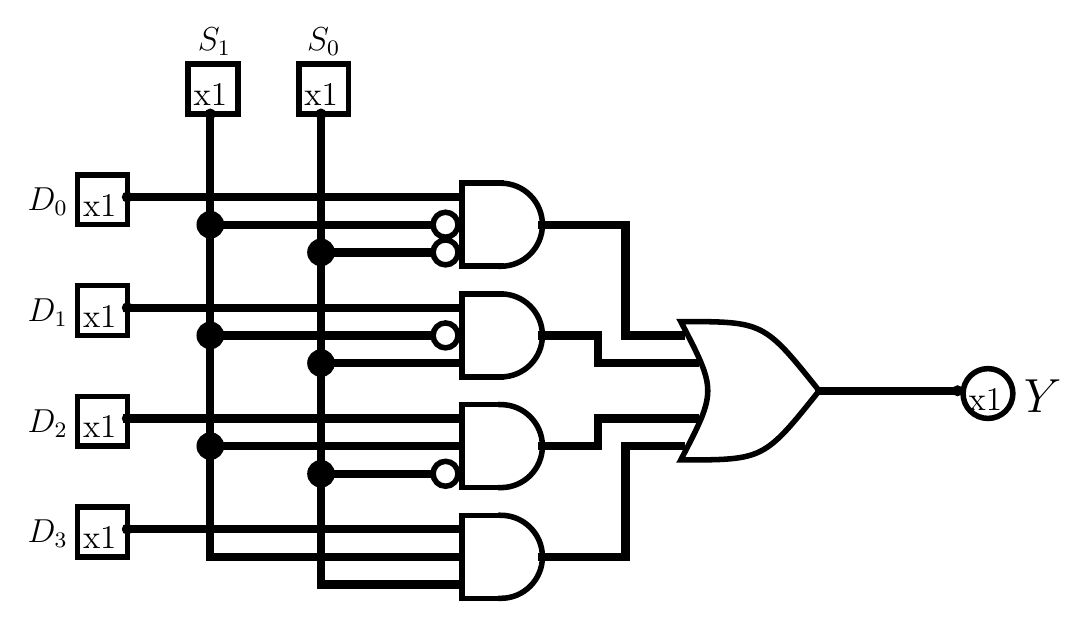
\begin{tikzpicture}[x=1pt,y=-1pt,line cap=rect]
\def\logisimfontA#1{\fontfamily{cmr}{#1}} % Replaced by logisim, original font was "SansSerif"
\def\logisimfontB#1{\fontfamily{Microsoft Sans Serif}{#1}}
\definecolor{custcol_0_0_0}{RGB}{0, 0, 0}
\definecolor{custcol_ff_ff_ff}{RGB}{255, 255, 255}
\draw [line width=3.0pt, custcol_0_0_0 ]  (46.0,74.0) -- (166.0,74.0) ;
\draw [line width=3.0pt, custcol_0_0_0 ]  (46.0,114.0) -- (166.0,114.0) ;
\draw [line width=3.0pt, custcol_0_0_0 ]  (46.0,154.0) -- (166.0,154.0) ;
\draw [line width=3.0pt, custcol_0_0_0 ]  (46.0,194.0) -- (166.0,194.0) ;
\draw [line width=3.0pt, custcol_0_0_0 ]  (296.0,144.0) -- (346.0,144.0) ;
\draw [line width=3.0pt, custcol_0_0_0 ]  (76.0,44.0) -- (76.0,84.0) -- (76.0,124.0) -- (76.0,164.0) -- (166.0,164.0) ;
\draw [line width=3.0pt, custcol_0_0_0 ]  (76.0,164.0) -- (76.0,204.0) -- (166.0,204.0) ;
\draw [line width=3.0pt, custcol_0_0_0 ]  (156.0,94.0) -- (116.0,94.0) -- (116.0,134.0) -- (166.0,134.0) ;
\draw [line width=3.0pt, custcol_0_0_0 ]  (116.0,134.0) -- (116.0,174.0) -- (156.0,174.0) ;
\draw [line width=3.0pt, custcol_0_0_0 ]  (116.0,174.0) -- (116.0,214.0) -- (166.0,214.0) ;
\draw [line width=3.0pt, custcol_0_0_0 ]  (116.0,44.0) -- (116.0,94.0) ;
\draw [line width=3.0pt, custcol_0_0_0 ]  (76.0,84.0) -- (156.0,84.0) ;
\draw [line width=3.0pt, custcol_0_0_0 ]  (76.0,124.0) -- (156.0,124.0) ;
\fill [line width=3.0pt, custcol_0_0_0]  (116.0,94.0) ellipse (5.0 and 5.0 );
\fill [line width=3.0pt, custcol_0_0_0]  (76.0,124.0) ellipse (5.0 and 5.0 );
\fill [line width=3.0pt, custcol_0_0_0]  (116.0,174.0) ellipse (5.0 and 5.0 );
\fill [line width=3.0pt, custcol_0_0_0]  (76.0,84.0) ellipse (5.0 and 5.0 );
\fill [line width=3.0pt, custcol_0_0_0]  (116.0,134.0) ellipse (5.0 and 5.0 );
\fill [line width=3.0pt, custcol_0_0_0]  (76.0,164.0) ellipse (5.0 and 5.0 );
\draw [line width=2.0pt, custcol_0_0_0 ]  (28.0,106.0) -- (45.0,106.0) ;
\draw [line width=2.0pt, custcol_0_0_0 ]  (46.0,106.0) -- (46.0,123.0) ;
\draw [line width=2.0pt, custcol_0_0_0 ]  (46.0,124.0) -- (29.0,124.0) ;
\draw [line width=2.0pt, custcol_0_0_0 ]  (28.0,124.0) -- (28.0,107.0) ;
\logisimfontA{\fontsize{12pt}{12pt}\selectfont\node[inner sep=0, outer sep=0, custcol_0_0_0, anchor=base west] at  (30.0,121.0)  {x1};}
\fill [line width=2.0pt, custcol_0_0_0]  (46.0,114.0) ellipse (2.0 and 2.0 );
\draw [line width=2.0pt, custcol_0_0_0 ]  (28.0,146.0) -- (45.0,146.0) ;
\draw [line width=2.0pt, custcol_0_0_0 ]  (46.0,146.0) -- (46.0,163.0) ;
\draw [line width=2.0pt, custcol_0_0_0 ]  (46.0,164.0) -- (29.0,164.0) ;
\draw [line width=2.0pt, custcol_0_0_0 ]  (28.0,164.0) -- (28.0,147.0) ;
\logisimfontA{\fontsize{12pt}{12pt}\selectfont\node[inner sep=0, outer sep=0, custcol_0_0_0, anchor=base west] at  (30.0,161.0)  {x1};}
\fill [line width=2.0pt, custcol_0_0_0]  (46.0,154.0) ellipse (2.0 and 2.0 );
\draw [line width=2.0pt, custcol_0_0_0 ]  (28.0,186.0) -- (45.0,186.0) ;
\draw [line width=2.0pt, custcol_0_0_0 ]  (46.0,186.0) -- (46.0,203.0) ;
\draw [line width=2.0pt, custcol_0_0_0 ]  (46.0,204.0) -- (29.0,204.0) ;
\draw [line width=2.0pt, custcol_0_0_0 ]  (28.0,204.0) -- (28.0,187.0) ;
\logisimfontA{\fontsize{12pt}{12pt}\selectfont\node[inner sep=0, outer sep=0, custcol_0_0_0, anchor=base west] at  (30.0,201.0)  {x1};}
\fill [line width=2.0pt, custcol_0_0_0]  (46.0,194.0) ellipse (2.0 and 2.0 );
\draw [line width=2.0pt, custcol_0_0_0 ]  (68.0,26.0) -- (85.0,26.0) ;
\draw [line width=2.0pt, custcol_0_0_0 ]  (86.0,26.0) -- (86.0,43.0) ;
\draw [line width=2.0pt, custcol_0_0_0 ]  (86.0,44.0) -- (69.0,44.0) ;
\draw [line width=2.0pt, custcol_0_0_0 ]  (68.0,44.0) -- (68.0,27.0) ;
\logisimfontA{\fontsize{12pt}{12pt}\selectfont\node[inner sep=0, outer sep=0, custcol_0_0_0, anchor=base west] at  (70.0,41.0)  {x1};}
\fill [line width=2.0pt, custcol_0_0_0]  (76.0,44.0) ellipse (2.0 and 2.0 );
\draw [line width=2.0pt, custcol_0_0_0 ]  (108.0,26.0) -- (125.0,26.0) ;
\draw [line width=2.0pt, custcol_0_0_0 ]  (126.0,26.0) -- (126.0,43.0) ;
\draw [line width=2.0pt, custcol_0_0_0 ]  (126.0,44.0) -- (109.0,44.0) ;
\draw [line width=2.0pt, custcol_0_0_0 ]  (108.0,44.0) -- (108.0,27.0) ;
\logisimfontA{\fontsize{12pt}{12pt}\selectfont\node[inner sep=0, outer sep=0, custcol_0_0_0, anchor=base west] at  (110.0,41.0)  {x1};}
\fill [line width=2.0pt, custcol_0_0_0]  (116.0,44.0) ellipse (2.0 and 2.0 );
\draw [line width=2.0pt, custcol_0_0_0]  (357.0,145.0) ellipse (9.0 and 9.0 );
\logisimfontA{\fontsize{12pt}{12pt}\selectfont\node[inner sep=0, outer sep=0, custcol_0_0_0, anchor=base west] at  (350.0,151.0)  {x1};}
\logisimfontA{\fontsize{16pt}{16pt}\fontseries{bx}\selectfont\node[inner sep=0, outer sep=0, custcol_0_0_0, anchor=base west] at  (370.0,152.0)  {$Y$};}
\fill [line width=2.0pt, custcol_0_0_0]  (346.0,144.0) ellipse (2.0 and 2.0 );
\draw [line width=2.0pt, custcol_0_0_0]  (161.0,84.0) ellipse (4.5 and 4.5 );
\draw [line width=2.0pt, custcol_0_0_0]  (161.0,94.0) ellipse (4.5 and 4.5 );
\draw [line width=2.0pt, custcol_0_0_0] (181.0,99.0) arc (90.0:-90.0:15.0 and 15.0 );
\draw [line width=2.0pt, custcol_0_0_0 ]  (181.0,69.0) -- (167.0,69.0) -- (167.0,99.0) -- (181.0,99.0) ;
\draw [line width=2.0pt, custcol_0_0_0]  (161.0,124.0) ellipse (4.5 and 4.5 );
\draw [line width=2.0pt, custcol_0_0_0] (181.0,139.0) arc (90.0:-90.0:15.0 and 15.0 );
\draw [line width=2.0pt, custcol_0_0_0 ]  (181.0,109.0) -- (167.0,109.0) -- (167.0,139.0) -- (181.0,139.0) ;
\draw [line width=2.0pt, custcol_0_0_0]  (161.0,174.0) ellipse (4.5 and 4.5 );
\draw [line width=2.0pt, custcol_0_0_0] (181.0,179.0) arc (90.0:-90.0:15.0 and 15.0 );
\draw [line width=2.0pt, custcol_0_0_0 ]  (181.0,149.0) -- (167.0,149.0) -- (167.0,179.0) -- (181.0,179.0) ;
\draw [line width=2.0pt, custcol_0_0_0] (181.0,219.0) arc (90.0:-90.0:15.0 and 15.0 );
\draw [line width=2.0pt, custcol_0_0_0 ]  (181.0,189.0) -- (167.0,189.0) -- (167.0,219.0) -- (181.0,219.0) ;
\draw [line width=3.0pt, custcol_0_0_0 ]  (196.0,84.0) -- (226.0,84.0) -- (226.0,124.0) -- (246.0,124.0) -- (246.0,124.0) ;
\draw [line width=3.0pt, custcol_0_0_0 ]  (196.0,124.0) -- (216.0,124.0) -- (216.0,134.0) -- (246.0,134.0) -- (251.0,134.0) ;
\draw [line width=3.0pt, custcol_0_0_0 ]  (196.0,164.0) -- (216.0,164.0) -- (216.0,154.0) -- (246.0,154.0) -- (251.0,154.0) ;
\draw [line width=3.0pt, custcol_0_0_0 ]  (246.0,164.0) -- (246.0,164.0) -- (226.0,164.0) -- (226.0,204.0) -- (196.0,204.0) ;
\draw [line width=2.0pt, custcol_0_0_0 ]  (296.0,144.0) .. controls  (276.0,119.0)  ..  (246.0,119.0) .. controls  (259.0,144.0)  ..  (246.0,169.0) .. controls  (276.0,169.0)  ..  (296.0,144.0) -- cycle ;
\draw [line width=2.0pt, custcol_0_0_0 ]  (28.0,66.0) -- (45.0,66.0) ;
\draw [line width=2.0pt, custcol_0_0_0 ]  (46.0,66.0) -- (46.0,83.0) ;
\draw [line width=2.0pt, custcol_0_0_0 ]  (46.0,84.0) -- (29.0,84.0) ;
\draw [line width=2.0pt, custcol_0_0_0 ]  (28.0,84.0) -- (28.0,67.0) ;
\logisimfontA{\fontsize{12pt}{12pt}\selectfont\node[inner sep=0, outer sep=0, custcol_0_0_0, anchor=base west] at  (30.0,81.0)  {x1};}
\fill [line width=2.0pt, custcol_0_0_0]  (46.0,74.0) ellipse (2.0 and 2.0 );
\logisimfontB{\fontsize{12pt}{12pt}\fontseries{bx}\selectfont\node[inner sep=0, outer sep=0, custcol_0_0_0, anchor=base west] at  (111.0,21.0)  {$S_0$};}
\logisimfontB{\fontsize{12pt}{12pt}\fontseries{bx}\selectfont\node[inner sep=0, outer sep=0, custcol_0_0_0, anchor=base west] at  (71.5,21.0)  {$S_1$};}
\logisimfontB{\fontsize{12pt}{12pt}\fontseries{bx}\selectfont\node[inner sep=0, outer sep=0, custcol_0_0_0, anchor=base west] at  (10.0,79.0)  {$D_0$};}
\logisimfontB{\fontsize{12pt}{12pt}\fontseries{bx}\selectfont\node[inner sep=0, outer sep=0, custcol_0_0_0, anchor=base west] at  (10.0,119.0)  {$D_1$};}
\logisimfontB{\fontsize{12pt}{12pt}\fontseries{bx}\selectfont\node[inner sep=0, outer sep=0, custcol_0_0_0, anchor=base west] at  (10.0,199.0)  {$D_3$};}
\logisimfontB{\fontsize{12pt}{12pt}\fontseries{bx}\selectfont\node[inner sep=0, outer sep=0, custcol_0_0_0, anchor=base west] at  (10.0,159.0)  {$D_2$};}
\end{tikzpicture}
}